\section{Обзор существующих решений}
\label{sec:Chapter2} \index{Chapter2}

\subsection{Формат сигнатур}

Прежде чем говорить непосредственно о методах автоматической генерации сигнатур, стоит сначала понять какие бывают сигнатуры и в каком формате они будут представлены.

Существует несколько представлений сигнатур. Некоторые из этих видов использовались для представлений сигнатур червей.
Однако для обычного трафика можно выделить два основных представления:

\begin{enumerate}
    \item сигнатуры, представленные регулярными выражениями
    \item сигнатуры, представленные строками
\end{enumerate}

Использование регулярных выражений для описания сигнатур приложений становится очень распространнённым в классификации потоков.
Однако процесс сопоставления регулярных выражений требует огромной вычислительной мощности, которая не масштабируется для идентификации сетевого трафика в режиме реального времени.
Способ построения регулярного выражения оказывает непосредственное влияние на классификацию потоков и на общую производительность сопоставления.
Несмотря на это, некоторые системы DPI используют регулярные выражения для представления сигнатур приложений. Система обнаружения/предотвращения вторжений Snort (IDS/IPS)
имеет более 1000 подписей приложений и предлагает пользователю возможность вставлять новые регулярные выражения по требованию.

Представление сигнатур в виде строк это компромисс между мощностью выражения и эффективностью сопоставления.
Также такой подход позволяет преобразовывать сигнатуры, представленные строками, в регулярные выражения.

Будем дальше рассматривать сигнатуры в виде строк, преобразование в регулярные выражения останется за рамками данной работы.

\subsection{Структура сигнатур}

Большинство форматов сигнатур в предыдущих работах представляют собой простые подстроки, которые часто появляются в полезной нагрузке.
Следовательно, всё ещё существует вероятность того, что извлеченные сигнатуры полезной нагрузки могут быть не специфичными для конкретного приложения,
некоторые могут принадлежать и другому приложению. Это называется избыточностью сигнатур.

Выделим три типа сигнатур:

\begin{enumerate}
    \item сигнатура содержимого (полезной нагрузки),
    \item сигнатура пакета,
    \item сигнатура потока.
\end{enumerate}

\begin{figure}[H]
    \begin{center}
        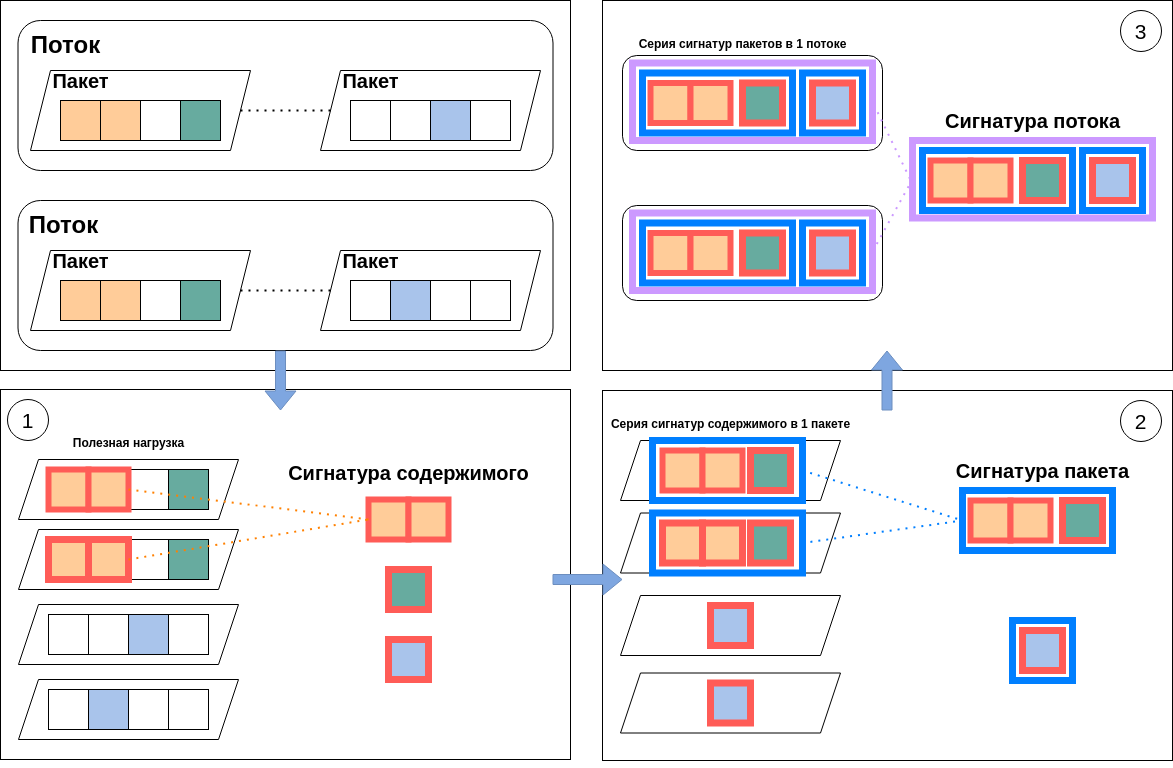
\includegraphics[width =\textwidth]{signature_structure.png}
        \caption{Процесс извлечения предлагаемой структуры сигнатур полезной нагрузки}
    \end{center}
\end{figure}

Сигнатура содержимого определяется как различимая и уникальная подстрока полезной нагрузки, состоящая из непрерывных символов или шестнадцатеричных значений.
На самом деле уникальность с помощью одной подстроки тяжело обеспечить, например, такие строки "GET" или "HTTP", которые часто встречаются в HTTP,
не могут служить конечными сигнатурами, так как они не различают приложения.

Сигнатура пакета состоит из серии сигнатур содержимого, которые появляются в одном пакете.
Так как классификация может выполняться без накопления пакетов, т.е. без сбора потока, то анализируется всегда хотя бы один пакет.
Это значит, что для классификации не имеет смысла использовать отдельно сигнатуру содержимого.

Сигнатура потока состоит из серии сигнатур пакетов, которые появляются в одном потоке, где под потоком понимается набор пакетов, имеющий одни и те же
IP-адресс источника, IP-адресс назначения, порт источника, порт назначения и используемый протокол транспортного уровня.
Сигнатура потока гораздо более специфична для конкретного приложения, чем сигнатура пакета, и значительно повышает точность.

\subsection{Метрики оценки качества сигнатур}

Для оценки качества получаемых сигнатур рассмотрим матрицу ошибок: 4 стандартные категории, к котором можно отнести результат работы классификатора на полученной сигнатуре.
В нашем случае рассматриваемый класс это целевой протокол или приложение.

\begin{table}[H]
\centering
\resizebox{\columnwidth}{!}{
\begin{tabular}{|c|c|c|}
\hline
                                                   & Принадлежит классу (P) & Не принадлежит классу (N) \\ \hline
Предсказана принадлежность классу (T)              & TP                     & TN                        \\ \hline
Предсказано отсутствие принадлежности к классу (F) & FP                     & FN                        \\ \hline
\end{tabular}
}
\end{table}

\subsection{Обзор существующих методов автоматической генерации сигнатур}

\newpage
